\addtocontents{toc}{\protect\setcounter{tocdepth}{1}}
\makeatletter
\addtocontents{toc}{%
  \begingroup
  \let\protect\l@chapter\protect\l@section
  \let\protect\l@section\protect\l@subsection
}
\makeatother


\chapter{Calendar interfaces} \label{a:calendars}

    \begin{figure}[ht]
        \centering
             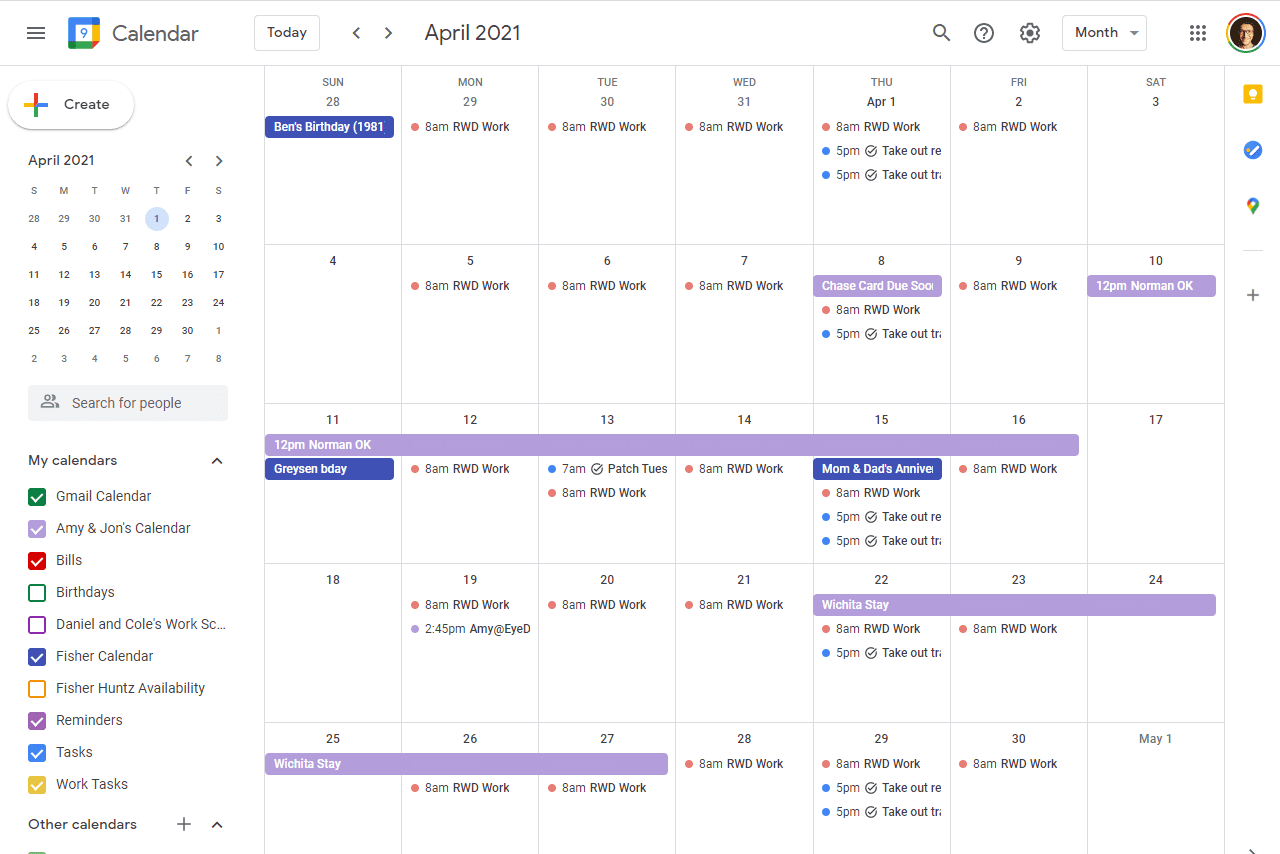
\includegraphics[width=0.95\textwidth]{figures/image14.png}
        \caption{Google Calendar interface} 
        \label{a:fig:gcalendar}
    \end{figure}
    
~
\footnote{https://www.lifewire.com/google-calendar-review-1357929}
\clearpage
        \begin{figure}[ht]
        \centering
             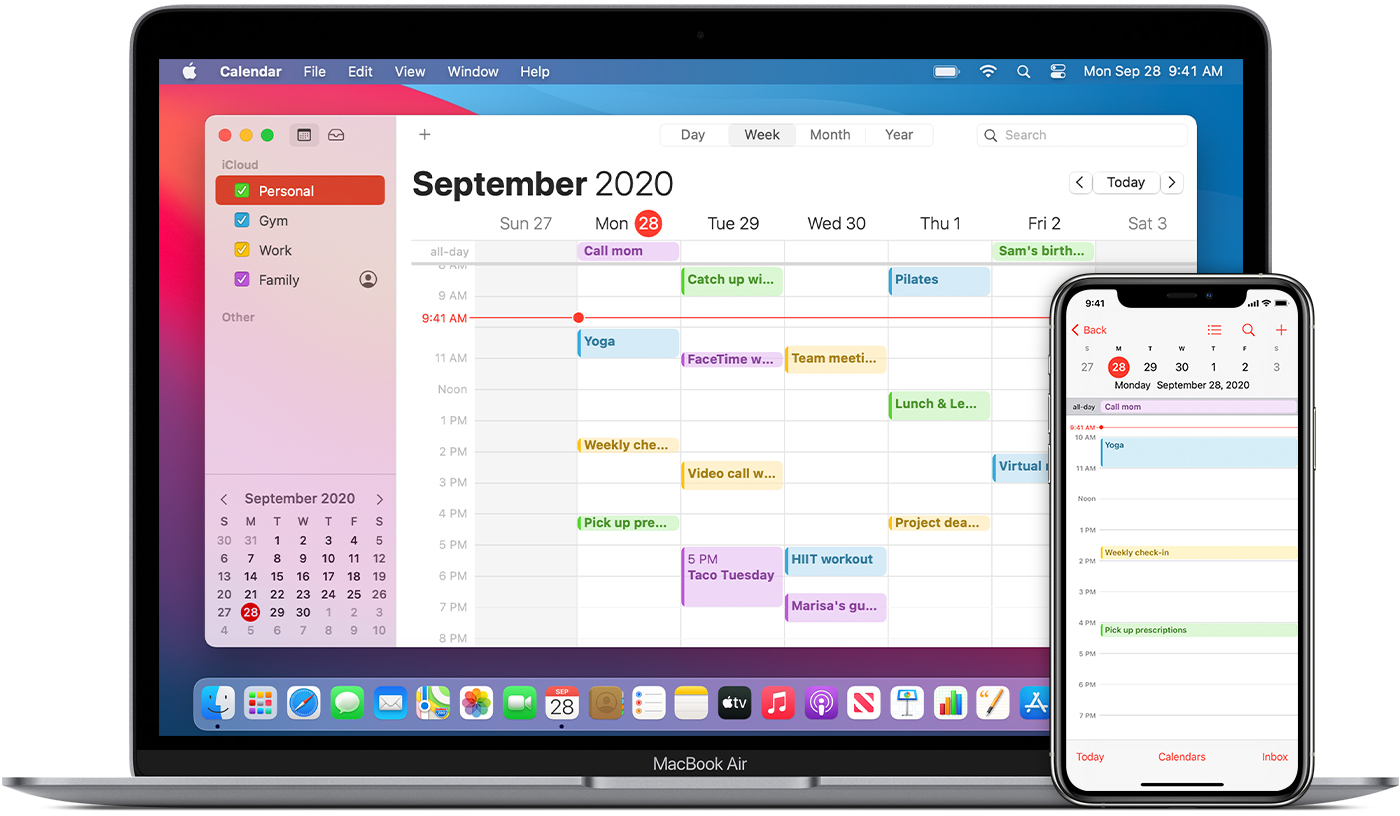
\includegraphics[width=0.95\textwidth]{figures/image6.jpg}
        \caption{Apple Calendar interface} 
        \label{a:fig:applecalendar}
    \end{figure}
    
    ~
    
    \footnote{https://support.apple.com/ro-ro/HT202337}

\chapter{UML diagrams} \label{b:uml}


    \begin{figure}[ht]
        \centering
             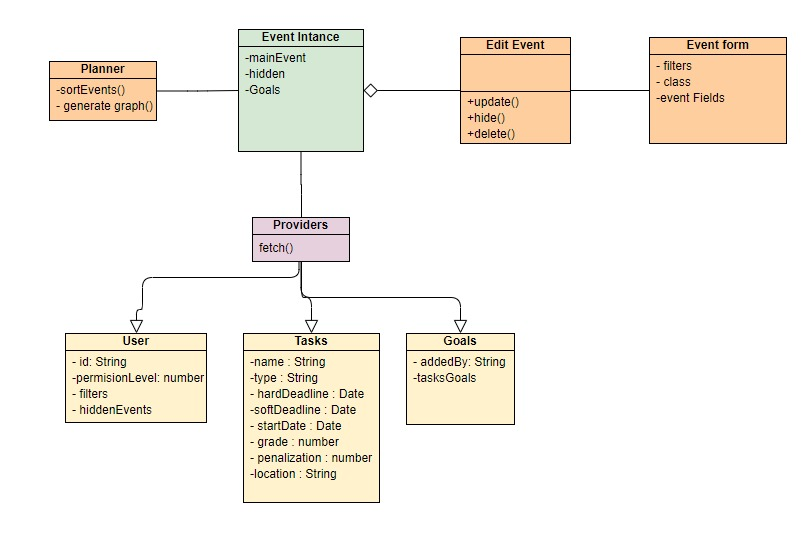
\includegraphics[width=0.95\textwidth]{figures/uml/structure.jpeg}
        \caption{Class diagram} 
        \label{b:fig:class}
    \end{figure}
    
    \begin{figure}[ht]
        \centering
             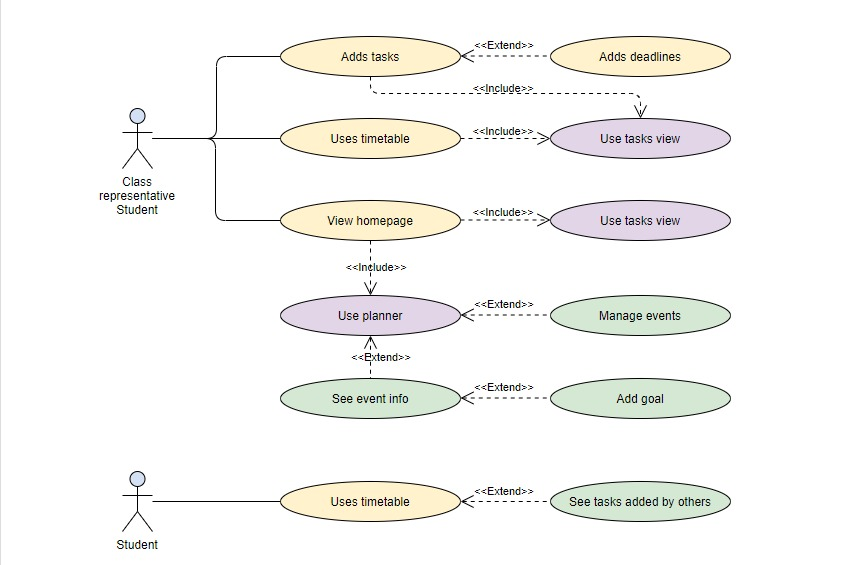
\includegraphics[width=0.95\textwidth]{figures/uml/usecase.jpeg}
        \caption{Use-case diagram} 
        \label{b:fig:usecase}
    \end{figure}
    
~